\chapter{Ground theory}
\section{Mail Transport}
Todays mail transport is mostly done via SMTP\index{SMTP} protocol as specified in \cite{RFC5321}. This protocol has proven to be stable and reliable. Most of the messages are passed from a MUA to a SMTP relay of a provider. From there the message is directly sent to the SMTP server of the recipient and from there to a server based storage of the recipient. The recipient may at any time connect to his server based storage and may optionally relocate the message to a client based (local) storage. The delivery from the server storage to the MUA of the recipient may happen by message polling or by message push (where as the later is usually implemented by a push-pull mechanism).\par

To understand the routing of a mail it is essential to understand the whole chain staring from a user(-agent) until arriving at the target user (and being read!). To simplify this I used a consistent model which includes all components (server and clients). The figure \ref{fig:MailAgents} shows all involved parties of a typical Mail routing. It is important to understand that Mail routing remains the same regardless of the used client. However -- Availability of a mail at its destination changes drastically depending on the type of client used. Furthermore control of the mail flow and control is different depending on the client.\par

\begin{figure}[htb]
  \centering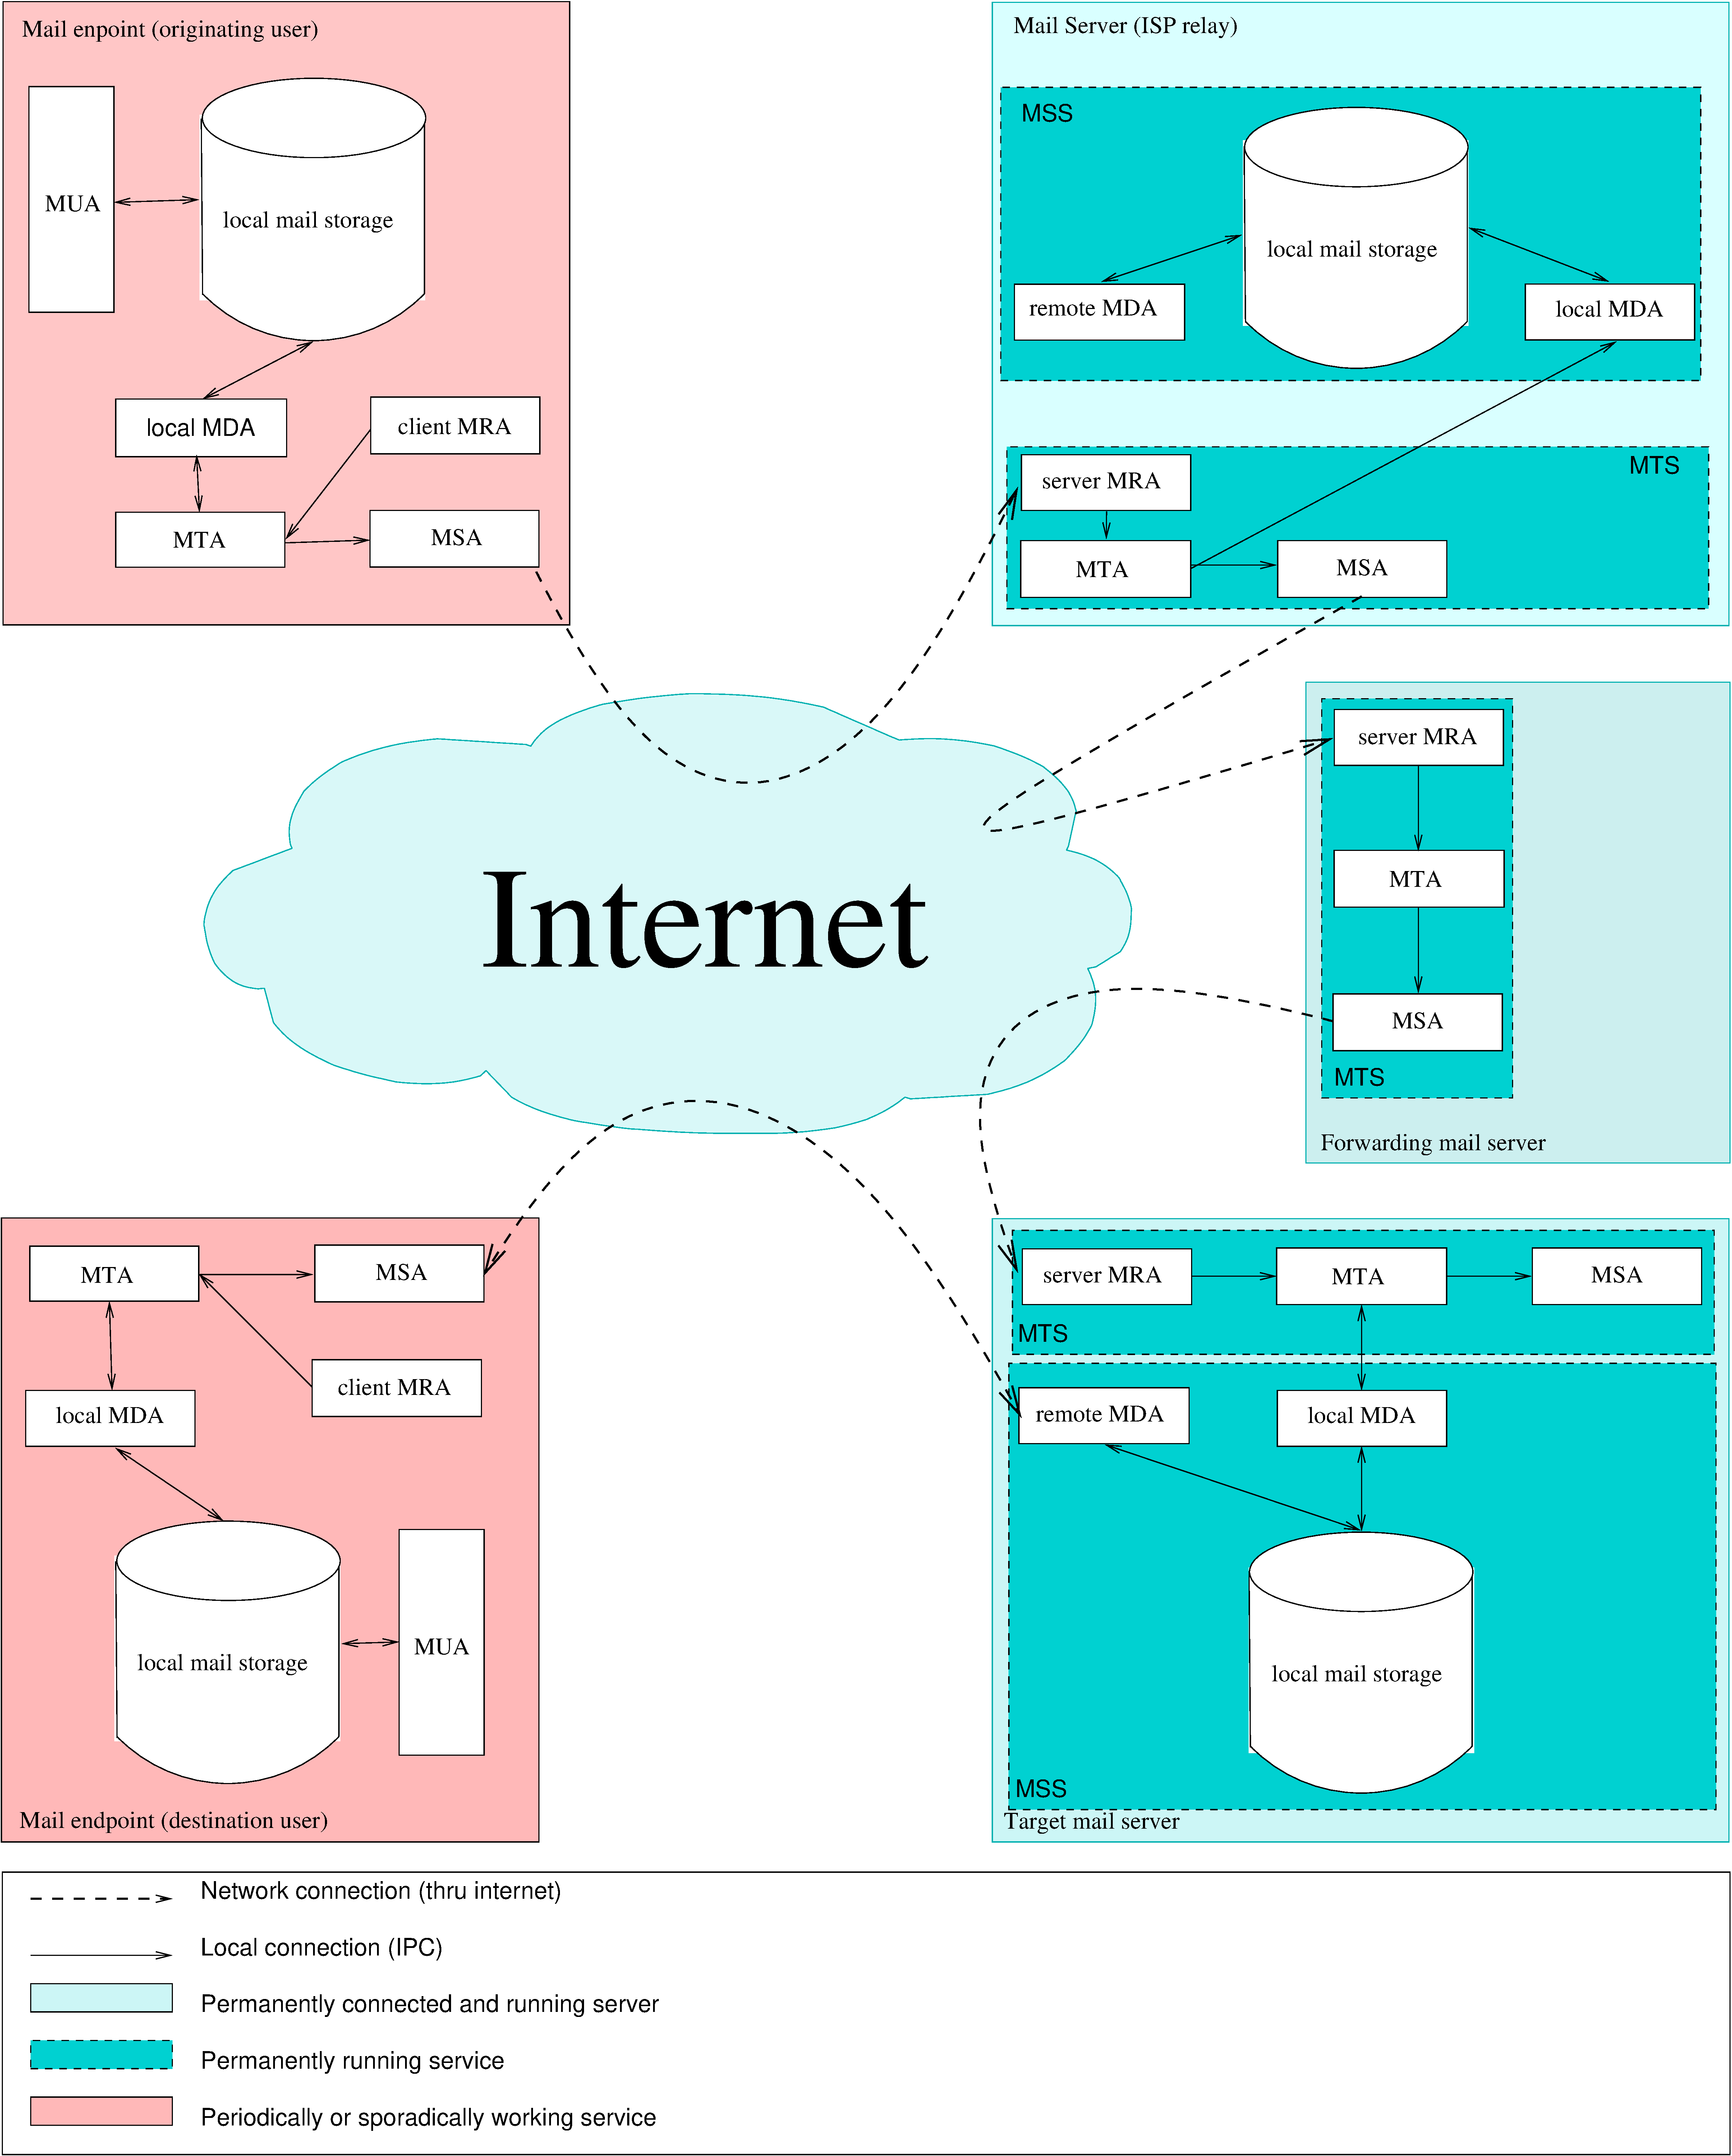
\includegraphics[width=\textwidth]{inc/MailAgents1}
  \caption{Mail Agents}
  \label{fig:MailAgents}
\end{figure}

Mails are typically initiated by a Mail User Agent (\defref{MUA}). A MUA accesses a local mail storage which may be the server storage or a local copy. The local copy may be a cache only copy, the only existing storage (when mails are fetched and deleted from the server after retrieval)  or a collected representation of multiple server storages (cache or authoritative).\par

Besides the MUA the only other component accessing a local mail storage is the Mail Delivery Agent (\defref{MDA}). An MDA is responsible for storing and fetching mails from the local mail storage. Mails destined for other accounts than the current one are forwarded to the MTA. In the case of a rich client the local MDA is part of the software provided by the user agent. In the case of a mail server the local MDA is part of the local Mailstore (not necessarily of the mail transport service).

On the server side there are usually two components (software sets) at work. A ``Mail Transport Service'' (\defref{MTS}) which consists generally of three parts. An server Message Receiving Agent (\defref{server MRA}) is typically a SMTP listening daemon. A Mail Transfer Agent (\defref{MTA}) which is responsible for routing and rewriting mails. 

\subsection{Mail clients}
\subsubsection{Fat clients}
\subsubsection{Server located clients}
\subsubsection{Web clients}

\section{Anonymity}
\subsection{\itshape{k}-anonymity}
\subsection{Plausible deniability}
\subsubsection{Deniable encryption}
\section{Identification and data signage}
\section{Encryption}
\subsection{Key exchange}
\subsubsection{Diffie-Hellmann key exchange}
\subsection{Symetric encryption}
\subsubsection{Advanced Encryption Standard}
\subsection{Asymetric encryption}
\subsubsection{RSA}
\subsubsection{El-Gamal}
\subsubsection{ECDSA}
\section{Mix cascades}
\section{Remailers}
Agents which do accept Mails from one party and forward it to another party while modifying its content well known under the name of ``Remailers''. Wi\-ki\-pe\-dia \cite{wiki:remailer} lists four types of Remailers.\par

Pseudonymous Remailers (or Type-0-Remailers) are remailers that establish a pseudonymity. This means that the senders Email-Address is removed and replaced by a pseudonymous E-Mailadress under the remailers control. This sender address may be used as an ordinary email-Adress to reeach the original sender of the mail. These types of Remailers allow to send mails while one or both recipients do not know their counterpart. The message (or at least parts of it) might be encrypted but do not have to be. For someone controling the Remailer it will always be possible to make a link between the pseudonymous mail address and a original mailadress. So pseudonymity is only granted towards people not controlling the remailer. Furthermore a person or organisation might be able to discover the Information tuple of Sender and pseudonymous email by analyzing messages and their timely context. So this remailer system is suspectible for traffic analysis.\par

Cypherpunk-Remailers (or Type-1-Remailers) do function a bit different. They take an encrypted message which was encrypted using the public key of the server, decrypt it and send it to a recipient. The original senders identity gets lost. A reply to a cypherpunk message is not possible. Messages sent to a cypherpunk server might contain messages to other cypherpunk remailers. This daisy-chaining of cypherpunk-nodes allows hiding the original sender-receiver-tuple from a single node. The first node knows only the the originating sender while the last node knows only the final recipient. All intermediate notes do only know the nodes they were linking. However if having traffic information of the entry and exit nodes the tuple might be discovered by traffic analysis.\par

Mixmaster remailer (or type-2-remailer) is a serie of mailers which split up a message into equally sized chunks and forward them using different paths (via SMTP) to an exit node where the message is reassembled and sent to the final recipient. However if having traffic information of the entry and exit nodes the tuple might be discovered by traffic analysis.\par

Mixminion remailer (or type-3-remailer) is an enhanced development of Mixmaster remailer. It is currently no longer under active development. It adresses serveral weaknesses of the mixmaster. Namely replies are possible. Forward anonymity is now given. Replay prevention and key rotation is part of the design and there are exit policies allowing ISPs to opt out from receiving remailer traffic. It is based on a proprietary communication network. It furthermore introduces dummy traffic to reduce traceability. This is the most complete approach email anonymity ever given. The aproach has however its weaknesses. To avoid partitioning attacks Miximinon distributes its network information with central redundant directory servers.\par

\section{Ethics}
\subsection{Human rights}
\subsubsection{Freedom of speech}
Article 19 of the ICCPR states that "everyone shall have the right to hold opinions without interference" and "everyone shall have the right to freedom of expression; this right shall include freedom to seek, receive and impart information and ideas of all kinds, regardless of frontiers, either orally, in writing or in print, in the form of art, or through any other media of his choice".

\subsection{Ethics of the Internet}
There is an RFC document regarding ``Ethics and the Internet''\cite[p.~1]{RFC1087}. Document states as unethical behaveour:
\begin{itemize}
\item An activity that seeks to gain unauthorized access to the resources of the Internet.
\item An activity that disrupts the intended use of the Internet.
\item An activity that wastes resources (people, capacity, computer) through such actions.
\item An activity that destroys the integrity of computer-based information.
\item An activity that compromises the privacy of users.
\end{itemize}
Unfortunately these actions do exist in modern internet and the most powerful players discovered so far are governmental agencies. Using a mixer and cryptographic algorithms definitely wastes resources. But it must be considered the right of every single user of the internet to uphold these points. As a final conclusion the proposed system does not violate the ethics of the internet but it must be designed to be as economically as possible with the existing resources.

\section{Possible legal issues}
One of the first questions I have been asked when working for this topic was: Is this legal? The question is important but not easy at all. The mail system is a global spanning network coming across almost any country of the world. Some of these countries consider almost any kind of secret as illegal as long as the country itself is not able to capture it. Some countries consider it as perfectly legal and some will generally accept its presence as long as the country or establishment is not endangered due to its usage. It is not part of this work to \par

My personal unscientific point is: I do not care. In my country it is definitely legal as long as I am a well behaved citizen (as long as I do not missuse this system to plan or do illegal actions). There are already proprietary systems available which offer the same functionality. All I do is adding this functionality to the common system instead of reinventing the wheel. There are however many very good reasons to have such a system. Correspondence about my health, my business relations, my friends or my family (to give just a couple of examples) should be kept private even in an open world. The misuse of information would cause tremendous damage and several events in time (which have been mentioned earlier) showed that there are many secret services and other players using any kind of information to achieve their own goals or the goals of associates. They do this regardless of any country borders or regulations. Since I have no means of controlling the flow of messages in the internet or the hubs where a mail is running thru I consider it as fair to generate an addon to compensate the lack of control in the existing system. Exactly as a car -- the system may be legal or illegal and it depends on the users whether he wants to use it or not and in what way.\par
